%Documento di proprietà di Vito Stefano Birardi™
%Qui sono presenti i package più comuni che usi, ricorda di usare solo quelli che ti servono 

%Variabili comuni
\newcommand{\Titolo}{Progetto Quality Treshold - Documentazione}
\newcommand{\Data}{\today}
\newcommand{\Materia}{}

%Comandi troppo lunghi da scrivere possono essere ri-operazionalizzati qui

\newcommand{\image}[3]{
    \begin{figure}[h!]
    \centering
    \includegraphics[width = 0.5 \textwidth]{#1}
    \caption{#2}
    \label{#3}
\end{figure}}

%Package per la formattazione del foglio

\documentclass[a4paper]{article}
\usepackage{amsmath}
\usepackage{amssymb}

%Package per la lingua dei capitoli

\usepackage[italian]{babel}

%Package per intestazione e pié di pagina

\usepackage{fancyvrb}
\usepackage{fancyhdr, lastpage}

%Package aggiuntivi 

\usepackage{cancel}
\usepackage{etoolbox}
\usepackage{xcolor}
\usepackage{subfig}
\usepackage{tikz, lmodern}
\usepackage[T1]{fontenc}
\usepackage[most]{tcolorbox}
\usepackage{graphicx}
\usepackage{hyperref}
\usepackage{parskip}
\usepackage{multicol}
\pagestyle{fancy}

%Formattazione hyperlinks

\hypersetup{
    colorlinks=true,
    linkcolor=blue,
    filecolor=magenta, 
    urlcolor=blue,
    pdfpagemode=FullScreen
}

%Formattazione di intestazione e pié di pagina

\lhead{\Data}
\rhead{Vito Stefano Birardi}
\lfoot{\Materia}
\rfoot{Pagina \thepage\ di \hyperlink{toc}{\pageref*{LastPage}}}
\renewcommand{\footrulewidth}{0.5pt}
\fancyfoot[C]{}
\patchcmd{\chapter}{\thispagestyle{plain}}{\thispagestyle{fancy}}{}

%Preambolo per prima pagina

\title{\Titolo}
\author{
    A cura di: 
    Vito Stefano Birardi
}
\date{\Data}

%Inizio documento vero e proprio


\begin{document}
\maketitle
\newpage
\hypertarget{toc}{\tableofcontents}
\newpage
\section{Introduzione}


Il progetto in questione utilizza l'algoritmo \textbf{Quality Threshold (QT)} per l'analisi dei dati. Tali dati possono essere estratti da un file o dalle tabelle di un database MySQL.

\section{Cos'è l'Algoritmo Quality Threshold}

L'algoritmo Quality Threshold è un algoritmo di \textbf{clustering} deterministico che appartiene alla famiglia degli algoritmi di raggruppamento gerarchico. A differenza degli algoritmi di partizionamento tradizionali, il QT non richiede di specificare a priori il numero di cluster da creare, ma si basa su un parametro di soglia di qualità (\textit{threshold}) che definisce il raggio massimo consentito per ogni cluster.

\section{Principio di Funzionamento}

L'algoritmo si basa sulla \textbf{minimizzazione della distanza} tra i punti dati e il centroide del cluster di appartenenza. Il processo di clustering avviene attraverso i seguenti passaggi:

\begin{enumerate}
\item \textbf{Selezione del punto candidato}: Per ogni punto del dataset, viene valutata la possibilità di creare un nuovo cluster
\item \textbf{Formazione del cluster}: Vengono raggruppati tutti i punti che si trovano entro il raggio di soglia specificato
\item \textbf{Selezione del cluster ottimale}: Viene scelto il cluster che contiene il maggior numero di punti
\item \textbf{Iterazione}: Il processo si ripete sui punti rimanenti fino a quando tutti i punti sono stati assegnati a un cluster
\end{enumerate}

\section{Caratteristiche Distintive}

L'algoritmo Quality Threshold presenta diverse caratteristiche che lo distinguono da altri approcci di clustering:

\subsection{Vantaggi}

\begin{itemize}
\item \textbf{Determinismo}: L'algoritmo restituisce sempre lo stesso risultato quando viene eseguito ripetutamente sullo stesso dataset, a differenza di algoritmi come il \textit{k-means} che possono produrre risultati diversi a seconda dell'inizializzazione casuale
\item \textbf{Numero di cluster automatico}: Non richiede di specificare il numero di cluster da creare, ma solo il raggio massimo (\textit{threshold}), rendendo l'algoritmo più flessibile per dataset con strutture sconosciute
\item \textbf{Robustezza al rumore}: È stato progettato per gestire efficacemente dati rumorosi e con distribuzioni non lineari
\item \textbf{Approccio gerarchico}: Utilizza una strategia gerarchica per la creazione dei cluster, garantendo una maggiore stabilità dei risultati
\end{itemize}

\subsection{Svantaggi}

\begin{itemize}
\item \textbf{Complessità computazionale}: Richiede una potenza di calcolo maggiore rispetto ad algoritmi di partizionamento come il \textit{k-means}, con una complessità temporale che può essere significativamente elevata per dataset di grandi dimensioni
\item \textbf{Sensibilità al parametro threshold}: La scelta del raggio di soglia influenza notevolmente la qualità del clustering ottenuto
\end{itemize}

\section{Ambiti di Applicazione}

L'algoritmo Quality Threshold è particolarmente adatto per contesti in cui:

\begin{itemize}
\item I dati presentano rumore significativo
\item La distribuzione dei dati è non lineare o presenta forme complesse
\item Non si conosce a priori il numero ottimale di cluster
\item È richiesta riproducibilità dei risultati
\item La qualità del clustering è più importante dell'efficienza computazionale
\end{itemize}
\section{Guida all'installazione}

Prima di essere in grado di eseguire il programma, è necessario eseguire il file \texttt{risorse.bat} contenuto nella cartella Risorse. 


Una volta eseguito il file, si aprirà una pagina di Powershell e seguirà un download.

\begin{figure}[h!]
    \centering
    
\includegraphics[width= 0.5\textwidth]{images/nuova docs.png}
    \caption{Schermatta di download}
\end{figure}

Al termine del download del file compresso delle risorse, verranno estratti i file necessari per l'esecuzione del programma.



Per il progetto in questione è necessario installare il Java Developer Kit (JDK) nella versione 22.0.1 e il software di gestione del database MySQL nella sua versione 8.0.39. 

La prima scheda di installazione che apparirà è quella del JDK. 

Verrà chiesto se si vuole eseguire l'installazione del JDK tramite permessi di amministratore, cliccare su \underline{Sì}.

\subsection{Installazione JDK}

Una volta confermata l'esecuzione come amministratore, si procederà all'installazione del JDK.

\begin{figure}[h!]
    \centering
    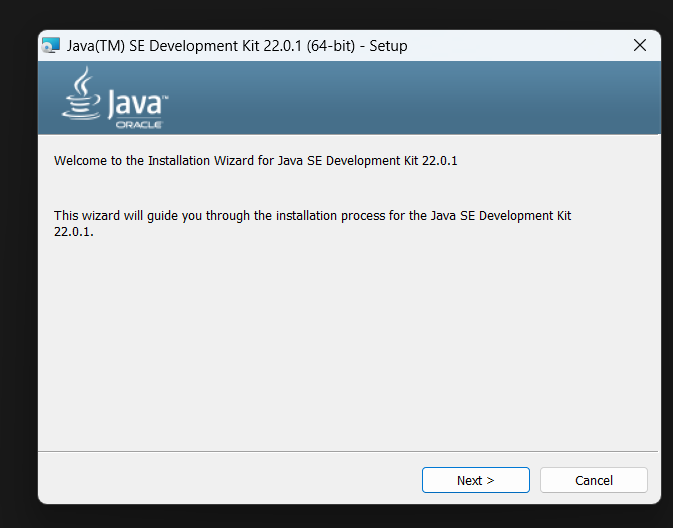
\includegraphics[width= 0.5\textwidth]{images/installazione java.png}
\end{figure}

Cliccare su \textbf{Avanti},nuovamente \textbf{Avanti} e infine, nel caso in cui l'installazione sia andata a buon fine, si dovràò cliccare sul tasto \textbf{Chiudi}.

\subsection{Variabili di ambiente}

è consigliato creare una variabile di ambiente per il JDK. Per farlo, si dovrà cercare la voce \textbf{variabili di ambiente} nella barra di ricerca di Windows e cliccare su {Modifica le variabili di ambiente per il tuo account}.

Successivamente si dovrà cliccare sul pulsante \textbf{Variabili di ambiente} e si aprirà una schermata con le variabili di ambiente. 



\begin{figure}[h!]
    \centering
    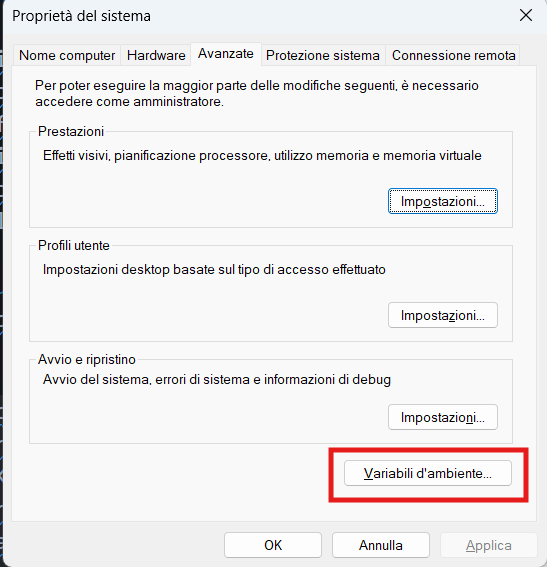
\includegraphics[width= 0.5\textwidth]{images/variabili ambienti.png}
    \caption{Schermata delle variabili di ambiente}
\end{figure}

Nella schermata, si dovra cliccare sulla variabile \texttt{PATH} e modificarla in modo da aggiungere il percorso del JDK, inserendo il percorso in cui è stato installato il JDK.

Una volta completata l'installazione del JDK, si procederà automaticamente con l'installazione del MySQL.



\subsection{Installazione MySQL}

Anche qui sarà necessario fornire i permessi di amministratore, cliccare dunque su \underline{Sì}.

\subsection{Schermata iniziale}

Dopodiché si aprirà la schermata di installazione di MySQL.

\begin{figure}[h!]
    \centering
    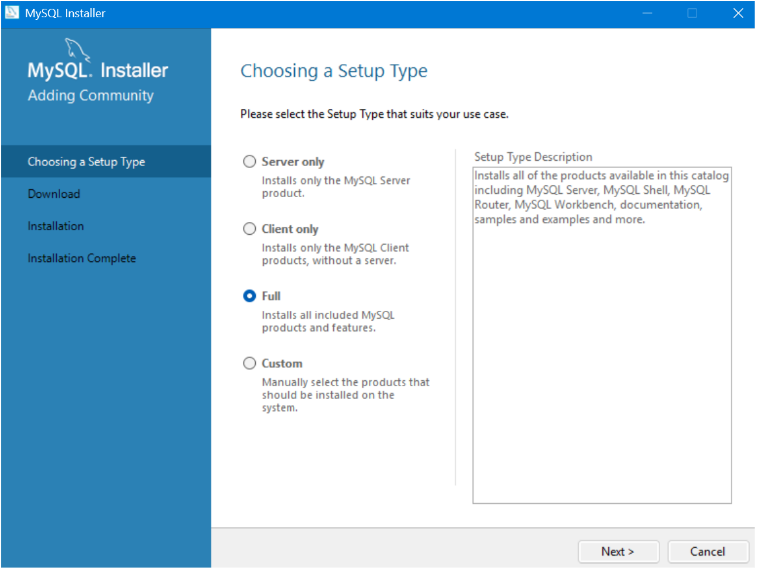
\includegraphics[width= 0.5\textwidth]{images/inizio mysql.png}
    \caption{Scelta del setup}
\end{figure}

Selezionare il tipo di setup \textbf{Full} e cliccare su \textbf{Next}. Tale scelta permetterà di installare tutti i componenti necessari per l'esecuzione del programma.

\subsection{Download dei file}

Si passerà alla schermata di download dei file necessari per l'installazione, cliccare su \textbf{Execute}. 

\begin{tcolorbox}[  colback=white!5!white, colframe=gray, title={Avvertenza} ]
    
    
    Tale schermata potrebbe richiedere un po' di tempo per il download dei file, a seconda della velocità della connessione internet. 
\end{tcolorbox}
    
Dopo aver scaricato i file, si dovrà cliccare nuovamente su \textbf{Execute}.

\begin{figure}[h!]
    \centering
    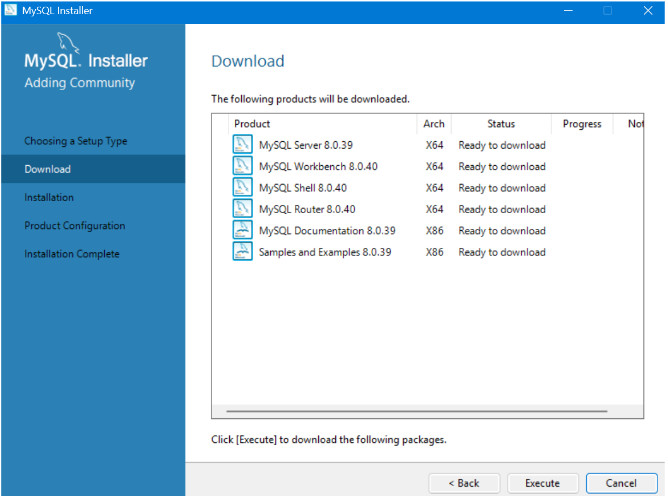
\includegraphics[width= 0.6\textwidth]{images/eexecute.png}
    \caption{Download MySQL}
\end{figure}

\subsection{Configurazione del account MySQL}
Una volta terminato il download, si procederà con la configurazione dell'account MySQL. Si dovrà quindi scegliere una password, necessaria per accedere al database. 


\begin{figure}[h!]
    \centering
    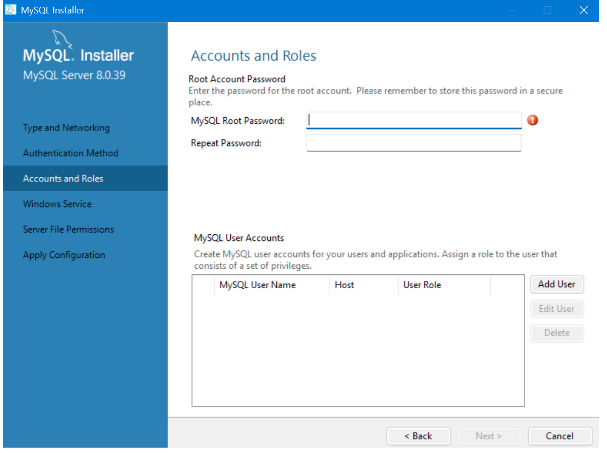
\includegraphics[width= 0.5\textwidth]{images/setup vero e proio musql.png}
    \caption{Configurazione account MySQL}
\end{figure}


Si giungerà infine alla scehermata di applicazione della configurazione del database. Cliccare su \textbf{Execute} per applicare la configurazione.

\begin{figure}[h!]
    \centering
    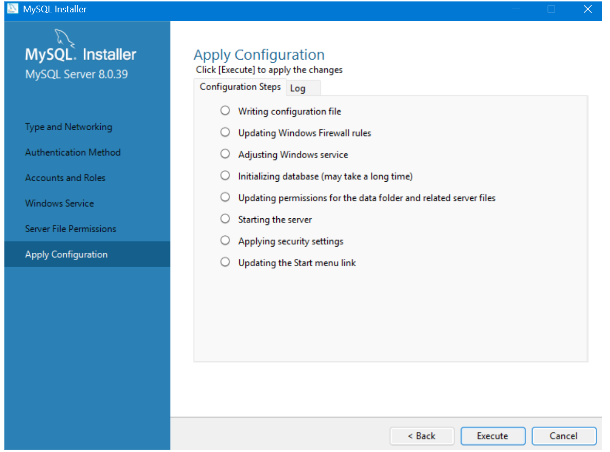
\includegraphics[width= 0.5\textwidth]{images/completamenot.png}
    \caption{Completamento installazione}
\end{figure}

Una volta terminata anche l'installazione del MySQL, si dovrà cliccare su \textbf{Finish} per chiudere l'installler. 

\begin{tcolorbox}[  colback=white!5!white, colframe=gray, title={Avvertenza} ]
    Per un corretto funzionamento sia del JDK che del MySQL, è consiglaito riavviare il computer.
    
\end{tcolorbox}


\subsection{Schermata finale}
Al termine dell'installazione il programma \texttt{resources.bat} mostrerà la seguente schermata. 

\begin{figure}[h!]
    \centering
    
\includegraphics[width= 0.6\textwidth]{images/insytllazione compeltata.png}
    \caption{Completamento installazione}
\end{figure}

\end{document}